\let\lesson\undefined
\newcommand{\lesson}{\phantomlesson{Bài 12.}}
\setcounter{section}{2}
\section{Bài tập tự luận}
\begin{enumerate}[label=\bfseries Bài \arabic*:,leftmargin=1.5cm]
	\item \mkstar{2}
	
	
	{
		Vật khối lượng $m$ đặt trên mặt phẳng nghiêng hợp với phương nằm ngang một góc $\alpha$. Hệ số ma sát trượt giữa vật và mặt phẳng nghiêng là $\mu_\text{t}$. Khi được thả ra, vật trượt xuống. Gia tốc của vật phụ thuộc vào những đại lượng nào?
		
	}
	
	\hideall
	{
		\begin{center}
			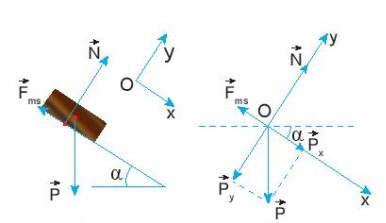
\includegraphics[scale=1]{../figs/VN10-2022-PH-TP021-3.jpg}
		\end{center}
		Theo định luật 2 Newton:
		
		$$ \vec F_\text{ms} + \vec P + \vec N = m\vec a.$$
		
		
		
		Áp dụng định luật 2 Newton theo hai trục Ox, Oy:
		
		$$\begin{cases}
			\text{Ox}:  mg\sin \alpha - \mu N= ma\ (1).\\
			\text{Oy}: 	N - mg\cos \alpha = 0\ (2).
		\end{cases}$$
		
		Thay (2) và (1) suy ra:
		
		$$a = g(\sin \alpha - \mu_\text{t} \cos \alpha).$$
	}
	
	\item \mkstar{2}
	
	
	{Cho hệ vật như hình. Biết $m_\text{A} > m_\text{B}$. Gia tốc của hai vật là $a$. Lực căng dây bằng bao nhiêu?
		\begin{center}
			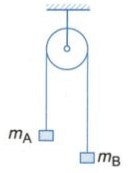
\includegraphics[scale=1]{../figs/VN10-2022-PH-TP021-22.jpg}
		\end{center}
	}
	
	\hideall{
		\begin{center}
			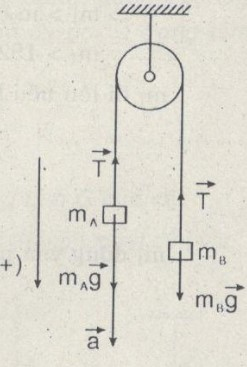
\includegraphics[scale=1]{../figs/VN10-2022-PH-TP021-23.jpg}
		\end{center}
		Áp dụng định luật II Newton cho vật $m_\text{A}$:
		
		$$m_\text{A} \vec a = m_\text{A} \vec g + \vec T$$
		
		Chiếu lên chiều dương ta được:
		
		$$ m_\text{A} a = m_\text{A} g - T \Rightarrow T = m_\text{A} (g-a).$$
	}
	
	\item \mkstar{3}
	
	
	{
		Một vật có khối lượng $m= \SI{2}{kg}$ đang nằm yên trên bàn nằm ngang thì được kéo bằng một lực có độ lớn $\SI{10}{N}$ theo hướng tạo với mặt phẳng ngang một góc $\alpha = 30^\circ$. Biết hệ số ma sát của vật với mặt sàn là 0,5. Tìm vận tốc của vật sau 5 giây kể từ lúc bắt đầu chịu lực tác dụng. Lấy $g = \SI{10}{m/s}^2.$
	}
	
	\hideall
	{
		\begin{center}
			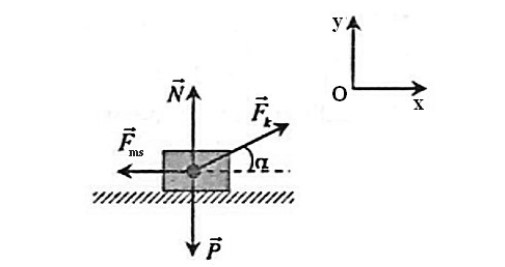
\includegraphics[scale=0.6]{../figs/VN10-2022-PH-TP021-7.jpg}
		\end{center}
		- Vật chịu tác dụng của trọng lực $P$, phản lực $N$, lực kéo $F$ và lực ma sát trượt $F_\text{ms}$. Chọn hệ trục Oxy như hình trên.
		
		- Áp dụng định luật II Newton ta có:
		
		$$\vec P + \vec N + \vec F + \vec F_\text{ms} = m\vec a.$$
		
		- Chiếu lên hệ trục ta được:
		
		$$\text{Ox}: F \cos \alpha - F_\text{ms} = ma.\ (1)$$
		
		$$\text{Oy}: - P + N + F \sin \alpha = 0 \Rightarrow N = P - F\sin \alpha.\ (2)$$
		
		$$F_\text{ms} = \mu N.\ (3)$$
		
		Từ (1), (2), (3) suy ra:
		
		$$a = \dfrac{F \cos \alpha - F_\text{ms}}{m} \approx \SI{0,58}{m/s}^2.$$
		
		Vận tốc của vật sau 5 giây
		
		$$v = at = \SI{2,9}{m/s}.$$
		
		
	}

	\item \mkstar{3}
	
	
	{
		Một học sinh dùng dây kéo một thùng sách nặng $\SI{10}{kg}$ chuyển động trên mặt sàn nằm ngang. Dây nghiêng một góc chếch lên trên $45^\circ$ so với phương ngang. Hệ số ma sát trượt giữa đáy thùng và mặt sàn là $\mu = \text{0,2}$ (lấy $g = \SI{9,8}{m/s}^2$). Hãy xác định độ lớn của lực kéo để thùng sách chuyển động thẳng đều.
	}
	
	\hideall
	{
		
		\begin{center}
			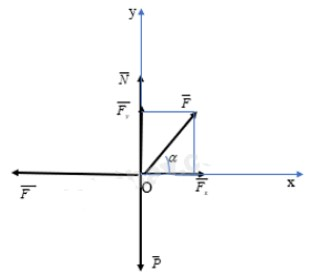
\includegraphics[scale=1]{../figs/VN10-2022-PH-TP021-12.jpg}
		\end{center}
		
		Theo định luật 2 Newton
		$$\vec F +\vec F_\text{ms} + \vec P + \vec N = m\vec a.$$
		
		Chiếu lên hệ trục tọa độ:
		
		$$\begin{cases}
			\text{Ox:} F_\text{x} - F_\text{ms} = ma \Leftrightarrow F\cos \alpha - \mu N = ma.\ (1) \\
			\text{Ox:}  N - P + F_\text{y}= 0 \Rightarrow N =P - F\sin \alpha\ (2).
			
		\end{cases}$$
		
		Mà $a = 0$ nên thay (2) vào (1) ta được:
		
		$$F\cos \alpha - \mu(P - F\sin \alpha) = 0 \Rightarrow F = \dfrac{\mu mg}{\cos \alpha + \mu \sin \alpha} \approx \SI{23,1}{N}.$$
		
		
	}

	\item \mkstar{3}
	
	
	{
		Một cái thùng khối lượng $m = \SI{40}{kg}$ đặt trên sàn nhà. Hệ số ma sát trượt giữa thùng và sàn nhà là $\mu_\text{t} = \SI{0,2}{}$. Người ta đẩy thùng bằng một lực $F =200N$ theo phương hợp với phương nằm ngang một góc $\alpha = 30^\circ$, chếch xuống phía dưới. Tính gia tốc của thùng. 
		
		\begin{center}
			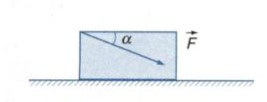
\includegraphics[scale=1]{../figs/VN10-2022-PH-TP021-17.jpg}
		\end{center}
	}
	
	\hideall
	{
		Vật chịu tác dụng của 4 lực được biểu diễn như hình vẽ.
		
		\begin{center}
			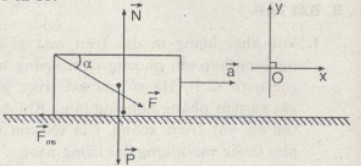
\includegraphics[scale=1]{../figs/VN10-2022-PH-TP021-18.jpg}
		\end{center}
		
		Áp dụng định luật II Newton ta có :
		
		$$\vec F + \vec F_\text{ms} + \vec P + \vec N = m\vec a.$$
		
		Chiếu lên hệ trục tọa độ $Oxy$:
		
		$$\begin{cases}
			Ox: F\cos \alpha - F_\text{ms} =ma.\qquad (1) \\
			Oy: - P + N - F\sin \alpha= 0 \Rightarrow N =mg + F \sin \alpha\qquad (2).
			
		\end{cases}$$
		
		Thay (2) vào (1) ta được:
		
		$$ a = \dfrac{F \cos \alpha - \mu (mg + F\sin \alpha)}{m} = \SI{1,87}{m/s}^2. $$
		
	} 

\item \mkstar{3}


{
	Từ chân một mặt phẳng nghiêng góc $30^\circ$ so với phương ngang, một chất điểm được truyền vận tốc đầu $\vec v_0$ hướng lên dọc theo mặt phẳng nghiêng. Hệ số ma sát giữa vật và mặt phẳng nghiêng là 0,5. Vật dừng lại ở đúng đỉnh của mặt phẳng nghiêng có độ cao $h =\SI{2}{m}.$ Lấy $ g = \SI{10}{m/s}^2$. Tìm $v_0$.
	
	\begin{center}
		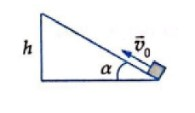
\includegraphics[scale=1]{../figs/VN10-2022-PH-TP021-9.jpg}
	\end{center}
}

\hideall
{
	
	Các lực tác dụng lên vật như hình vẽ.
	\begin{center}
		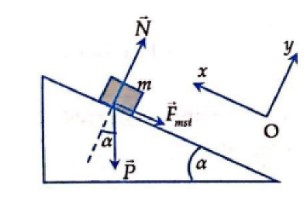
\includegraphics[scale=1]{../figs/VN10-2022-PH-TP021-10.jpg}
	\end{center}
	Áp dụng định luật II Newton:
	
	$$\vec N + \vec P + \vec F_\text{ms} = m\vec a.\ (1)$$
	
	Chọn hệ trục tọa độ Oxy như hình vẽ.
	
	Chiếu (1) lên Oy ta có:
	
	$$ - P \cos \alpha + N =0 \Rightarrow N = mg \cos \alpha\ (2).$$
	
	Chiếu (1) lên Ox ta có: 
	
	$$ - P \sin \alpha - F_\text{ms} = ma\ (3).$$
	
	Từ (2) và (3) suy ra:
	
	$$a = -g(\sin \alpha + \mu \cos \alpha).$$
	
	Quãng đường vật đi được chính bằng chiều dài mặt phẳng nghiêng:
	
	$$s = \dfrac{h}{\sin \alpha } = \SI{4}{m}.$$
	
	Áp dụng công thức:
	
	$$v^2 - v_0^2 = 2as\qquad (v=0)$$ 
	
	Suy ra:
	
	$$v_0 = \sqrt{2g(\sin \alpha + \mu \cos \alpha)s} \approx \SI{8,6}{m/s}.$$
}

	
\item \mkstar{3}


{Một vật đang chuyển động trên đường nằm ngang với vận tốc $\SI{15}{m/s}$ thì trượt lên một cái dốc dài $\SI{100}{m}$ cao $\SI{10}{m}$. Biết hệ số ma sát giữa vật và mặt dốc là $\mu = \SI{0.05}{}$. Lấy $g=\SI{10}{m/s^2}$. Tính quãng đường vật đi được từ chân dốc cho đến điểm cao nhất có thể và tốc độ của nó khi trở lại chân dốc.
}

\hideall
{Góc nghiêng của mặt phẳng nghiêng:
	$$\sin \alpha = \dfrac{10}{100} = \dfrac{1}{10} \Rightarrow \cos \alpha = \dfrac{3\sqrt{11}}{10}$$
	
	Độ lớn phản lực trên phương vuông góc mặt nghiêng:
	$$N=mg \cos \alpha = mg \cdot \dfrac{3\sqrt{11}}{10}$$
	
	Độ lớn của trọng lực trên phương song song mặt nghiêng:
	$$P_x = mg \sin \alpha = mg \cdot \dfrac{1}{10}$$
	
	Tổng hợp lực gây ra gia tốc cho vật:
	$$-P_x - F_\text{ms} = ma \Rightarrow a =\SI{-1.5}{m/s^2} $$
	
	Quãng đường vật trượt trên mặt nghiêng cho đến khi vật ở điểm cao nhất:
	$$2aS = 0 -v^2 \Rightarrow S = \SI{75}{m}$$
	
	Gia tốc khi vật đi xuống:
	$$P_x - F_\text{ms} = ma' \Rightarrow a' = \SI{0.5}{m/s^2}$$
	
	Tốc độ của vật khi ở chân dốc:
	$$2a' S = v'^2 - 0 \Rightarrow v' = \SI{8.66}{m/s}$$
}

\item \mkstar{3}


{
	Một thùng hàng trọng lượng $\SI{500}{N}$ đang trượt xuống dốc. Mặt dốc tạo với phương ngang một gốc $30^\circ$. Chọn hệ tọa độ vuông góc $Oxy$ sao cho trục $Ox$ theo hướng chuyển động của thùng.
	\begin{enumerate}[label=\alph*)]
		\item  Vẽ giản đồ vecto lực tác dụng lên thùng.
		\item Tính các thành phần của trọng lực theo các trục tọa độ vuông góc.
		\item Giải thích tại sao lực pháp tuyến của dốc lên thùng hàng không có tác dụng kéo thùng hàng xuống dốc.
		\item Xác định hệ số ma sát trượt giữa mặt dốc và thùng hàng nếu đo được gia tốc chuyển động của thùng là $\SI{2}{m/s}^2$. Bỏ qua lực cản của không khí lên thùng.
	\end{enumerate}
}

\hideall
{
	
	\begin{enumerate}[label=\alph*)]
		\item  Vẽ giản đồ vecto lực tác dụng lên thùng.
		
		
		\begin{center}
			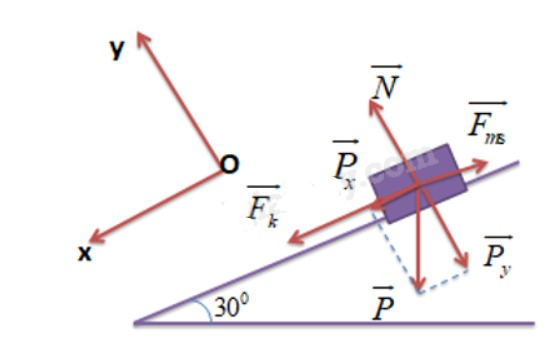
\includegraphics[scale=0.5]{../figs/VN10-2022-PH-TP021-14.jpg}
		\end{center}
		
		\item 
		Ta có:
		$$\begin{cases}
			P_\text{x}= P\sin \alpha = \SI{250}{N}.   \\
			P_\text{y}= P \cos \alpha = \xsi{250\sqrt 3}{N}.
		\end{cases}$$
		
		\item Lực pháp tuyến của dốc lên thùng hàng không có tác dụng kéo thùng hàng xuống dốc vì nó cân bằng với thành phần $\vec P_\text{y}$
		của trọng lực.
		
		
		\item Theo định luật 2 Newton
		$$\vec F_\text{ms} + \vec P + \vec N = m\vec a.$$
		
		Chiếu lên hệ trục tọa độ:
		
		$$\begin{cases}
			Ox: P_\text{x} - F_\text{ms} =ma \Leftrightarrow  P_\text{x} - \mu N = ma.\qquad (1) \\
			Oy: N - P_\text{y}= 0 \Rightarrow N =P_\text{y}\qquad (2).
			
		\end{cases}$$
		
		Thay (2) vào (1) ta được:
		
		$$ P_\text{x} - \mu P_\text{y} = ma \Rightarrow \mu = \dfrac{ P_\text{x}  -ma}{ P_\text{y}} \approx 0,346 $$
	\end{enumerate}
}

\item \mkstar{3}


{
	Hai vật có khối lượng lần lượt là $m_1 = \SI{5}{kg}$ và $m_2 = \SI{10}{kg}$ được nối với nhau bằng một sợi dây không dãn và được đặt trên một mặt sàn nằm ngang. Kéo vật 1 bằng một lực $\vec F$ nằm ngang có độ lớn $F = \SI{45}{N}$. Hệ số ma sát giữa mỗi vật và mặt sàn là $\mu = \text{0,2}$. Lấy $g = \SI{9,8}{m/s}^2$. Tính gia tốc của mỗi vật và lực căng của dây nối.
}

\hideall
{
	\begin{center}
		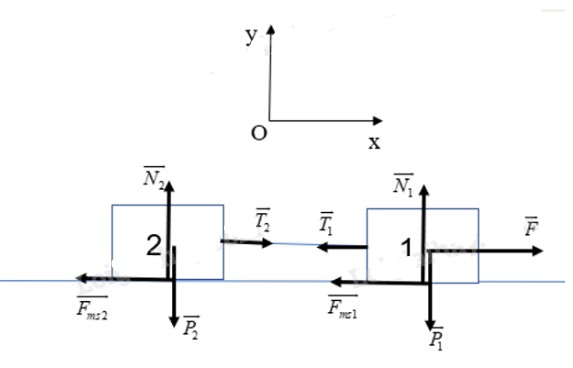
\includegraphics[scale=0.8]{../figs/VN10-2022-PH-TP021-13.jpg}
	\end{center}
	
	
	Chọn hệ quy chiếu như hình vẽ.
	
	Theo định luật 2 Newton cho hệ vật, ta có:
	
	$$\vec P_1 + \vec P_2 + \vec N_1 + \vec N_2 + \vec F + \vec F_\text{ms1} + \vec F_\text{ms2} + \vec T_1 + \vec T_2 = (m_1 + m_2)\vec a.\ (*)$$
	
	Chiếu (*) lên Ox, ta có
	
	$$F - F_\text{ms1} - F_\text{ms2} - T_1 + T_2 = (m_1 + m_2)a. \Rightarrow F - \mu(N_1 + N_2) = (m_1 + m_2)a\Rightarrow a = \dfrac{F - \mu (N_1 + N_2)}{m_1+m_2}\ (1).$$
	
	Chiếu (*) lên Oy, ta có
	
	$$N_1 + N_2 - P_1 - P_2 =0 \Rightarrow N_1 + N_2 = P_1 + P_2 \Rightarrow N_1 + N_2 = (m_1 + m_2)g\ (2).$$
	
	Thay (2) vào (1) ta được:
	
	$$a = \dfrac{F - \mu (m_1 + m_2)g}{m_1+m_2}= \SI{1,04}{m/s}^2.$$
	
	Theo định luật 2 Newton, ta có
	
	$$\vec P_1 + \vec N_1 + \vec F + \vec F_\text{ms1} + \vec T_1 = m_1 \vec a\ (**).$$
	
	Chiếu (**) lên Ox, ta có:
	
	$$F - F_\text{ms1} - T_1 = m_1a.\ (3)$$
	Chiếu (**) lên Oy, ta có:
	
	$$N_1 = P_1 = m_1g. \ (4)$$
	
	Thay (4) vào (3) suy ra:
	
	$$T_1 = F - \mu m_1 g - m_1 a  = \SI{30}{N}.$$
	
	
}

\item \mkstar{3}


{
	Hai vật $m_1 = \SI{1}{kg}$, $m_2 = \SI{0,5}{kg}$ nối với nhau bằng sợi dây và được kéo lên thẳng đứng nhờ lực $F = \SI{18}{N}$ đặt lên vật I. Tìm gia tốc chuyển động. Coi dây là không giãn và có khối lượng không đáng kể.
	\begin{center}
		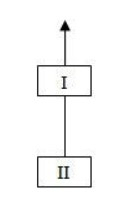
\includegraphics[scale=0.8]{../figs/VN10-2022-PH-TP021-8.jpg}
	\end{center}
}

\hideall
{
	Các ngoại lực tác dụng lên hệ: các trọng lực $\vec P_1$, $\vec P_2$, lực kéo $\vec F$.
	
	Chọn chiều dương hướng lên. Gia tốc của hệ là:
	
	$$a = \dfrac{F - P_1 - P_2}{m_1 + m_2} = \SI{2}{m/s}^2.$$
}

\item \mkstar{3}


{
	Người ta vắt qua một chiếc ròng rọc nhẹ một đoạn dây, ở hai đầu có treo hai vật A và B có khối lượng là $m_\text{A} =\SI{260}{g}$ và $m_\text{B} = \SI{240}{g}$ . Thả cho hệ bắt đầu chuyển động. Tính gia tốc của hệ vật.
	
	\begin{center}
		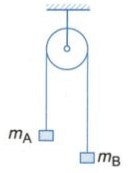
\includegraphics[scale=1]{../figs/VN10-2022-PH-TP021-22.jpg}
	\end{center}
}

\hideall{
	\begin{center}
		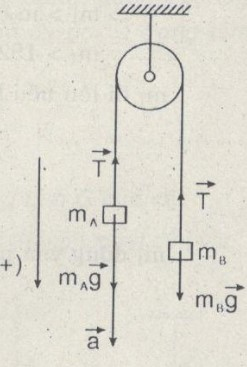
\includegraphics[scale=0.6]{../figs/VN10-2022-PH-TP021-23.jpg}
	\end{center}
	
	Chọn chiều dương là chiều chuyển động của hai vật.
	
	Áp dụng định luật II Newton:
	
	$$\vec P_1 + \vec T_1 = m_1 \vec a \Rightarrow P_1 - T_1 = m_1a\ (1).$$
	
	$$\vec P_2 + \vec T_2 = m_2 \vec a \Rightarrow - P_2 - T_2 = m_2a\ (2).$$
	
	Lấy (1) cộng (2) vế theo vế
	
	$$ P_1 - P_2 = m_1 a + m_2 a = (m_1+ m_2)a \Rightarrow a = \dfrac{P_1 - P_2}{m_1 + m_2} = \SI{0,4}{m/s}^2.$$
	
}


\item \mkstar{4}


{Cho cơ hệ như hình vẽ.
	\begin{center}
		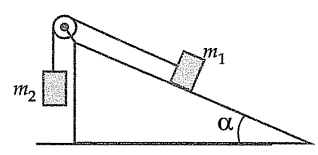
\includegraphics[scale=0.8]{../figs/VN10-2021-PH-TP012-3.png}
	\end{center}
	Mặt phẳng nghiêng cố định, nghiêng góc $\alpha$ so với phương ngang. Hai chất điểm khối lượng $m_1$, $m_2$ được nối với nhau bởi dây nhẹ, không dãn vắt qua ròng rọc nhẹ có kích thước không đáng kể. Biết rằng $m_2 > m_1 \sin \alpha$. Bỏ qua mọi ma sát, cho gia tốc trọng trường là $g$. Thả hai vật chuyển động tự do, tìm gia tốc của mỗi vật.
}

\hideall
{	\begin{center}
		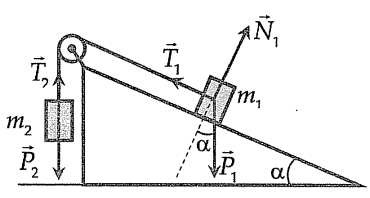
\includegraphics[scale=0.8]{../figs/VN10-2021-PH-TP012-4.png}
	\end{center}
	
	Do $m_2 > m_1 \sin \alpha$ nên $m_2$ sẽ đi xuống.
	
	Áp dụng định luật II Newton cho mỗi vật:
	\begin{align*}
		\vec T_1 + \vec N + \vec P_1 &= m_1 \vec a_1 \\
		\vec T_2 + \vec P_2 &= m_2 \vec a_2
	\end{align*}
	
	Do dây nhẹ, không dãn, ròng rọc không khối lượng nên $T_1 = T_2 = T$, $a_1 = a_2 = a$.
	
	Chiếu các vectơ lên phương chuyển động của mỗi vật, ta được:
	\begin{align*}
		T - P_1 \sin \alpha &= m_1 a \\
		-T + P_2 &= m_2 a
	\end{align*}
	
	Suy ra $a=\dfrac{m_2 - m_1 \sin \alpha}{m_1 + m_2}g$.
	
	\textit{(*) Có thể xét chuyển động của cả hệ để giải.}
}

\item\mkstar{4}\\
{\begin{minipage}[l]{0.7\textwidth}
		Cho hệ vật như vẽ. Hai vật nặng cùng khối lượng $m_1=m_2=\SI{1}{\kilogram}$ có độ cao chênh nhau một khoảng $\SI{2}{\meter}$. Đặt thêm vật $m_3=\SI{500}{\gram}$ lên vật $m_1$, bỏ qua ma sát, khối lượng của dây và ròng rọc. Tìm vận tốc của các vật khi hai vật $m_1$ và $m_2$ ở ngang nhau. Cho $g=\SI{10}{\meter/\second^2}$.
	\end{minipage}
	\begin{minipage}{0.3\textwidth}
		\begin{center}
			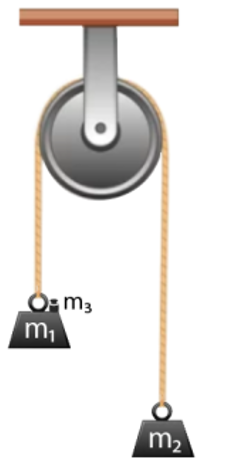
\includegraphics[width=0.3\linewidth]{../figs/VN10-2022-PH-TP021-P-1}
		\end{center}
	\end{minipage}
}
\hideall{
\begin{center}
	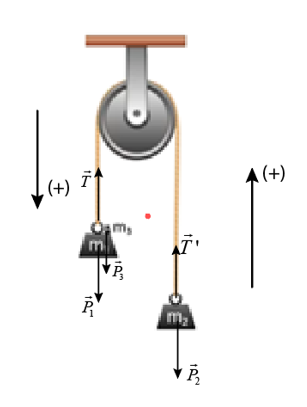
\includegraphics[width=0.3\linewidth]{../figs/VN10-2022-PH-TP021-P-2}
\end{center}
Vì $\left(m_1+m_3\right)>m_2$ nên $m_1$ và $m_3$ đi xuống và $m_2$ đi lên.\\
Chọn chiều dương là chiều chuyển động của hệ vật.\\
Ngoại lực tác dụng lên hệ gồm: $\overrightarrow{P_1}$, $\overrightarrow{P_3}$, $\overrightarrow{P_2}$.\\
Áp dụng định luật II Newton lên hệ:
$$\overrightarrow{P_1}+\overrightarrow{P_3}+\overrightarrow{P_2}=\left(m_1+m_2+m_3\right)\vec{a}$$
Chiếu phương trình trên lên chiều dương:
$$g\left(m_1+m_3-m_2\right)=\left(m_1+m_2+m_3\right)a$$
$$\Rightarrow a=\dfrac{\left(m_1+m_3-m_2\right)g}{m_1+m_2+m_3}=\SI{2}{\meter/\second^2}.$$
Khi hai vật ngang nhau, mỗi vật đã đi được theo chiều dương một quãng đường $s=\dfrac{h}{2}=\SI{1}{\meter}$.\\
Vận tốc của các vật lúc này: 
$$v=\sqrt{2as}=\SI{2}{\meter/\second}.$$
}

\item\mkstar{4}\\
{Cho cơ hệ như hình vẽ. Vật thứ nhất có khối lượng $m_1=\SI{1}{\kilogram}$, vật thứ hai có khối lượng $m_2=\SI{3}{\kilogram}$ nối với nhau bởi một sợi dây nhẹ, không dãn. Biết hệ số ma sát trượt giữa hai vật và mặt phẳng ngang là $\mu=0,1$. Tác dụng vào A một lực kéo $F=\SI{5}{\newton}$ theo phương hợp với phương ngang một góc $\alpha=\SI{30}{\degree}$. Lấy $g =\SI{9.8}{\meter/\second^2}$. Tìm lực căng của dây nối hai vật.
	\begin{center}
		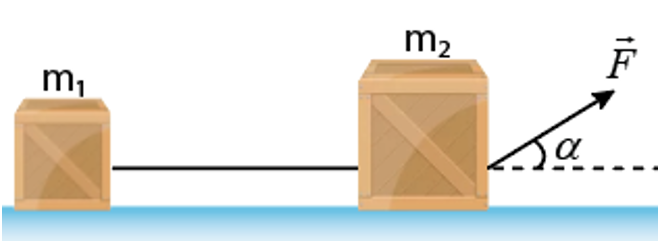
\includegraphics[width=0.3\linewidth]{../figs/VN10-2022-PH-TP021-P-3}
	\end{center}  

}
\hideall{
	\begin{center}
		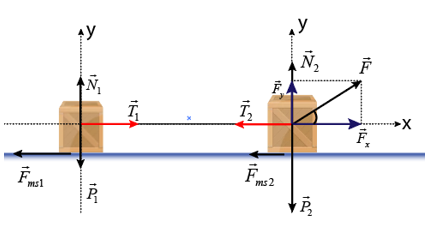
\includegraphics[width=0.5\linewidth]{../figs/VN10-2022-PH-TP021-P-4}
	\end{center}  
Ngoại lực tác dụng lên hệ vật gồm: $\overrightarrow{P_1}, \overrightarrow{N_1}, \overrightarrow{F_{ms 1}}, \overrightarrow{P_2}, \overrightarrow{N_2}, \overrightarrow{F_{ms 2}}, \overrightarrow{F}$.\\
Áp dụng định luật II Newton cho hệ:
$$\overrightarrow{P_1}+ \overrightarrow{N_1}+ \overrightarrow{F_{ms 1}}+ \overrightarrow{P_2}+ \overrightarrow{N_2}+\overrightarrow{F_{ms 2}}+\overrightarrow{F}=\left(m_1+m_2\right)\vec{a}$$
Chiếu phương trình trên lên chiều chuyển động ta có:
$$F\cdot\cos\alpha-F_{ms 1}-F_{ms 2}=\left(m_1+m_2\right)a$$
$$\Leftrightarrow F\cdot\cos\alpha -\mu m_1g-\mu \left(m_2g-F\sin\alpha\right)=\left(m_1+m_2\right)a$$
$$\Rightarrow a=\dfrac{F\cos\alpha -\mu g\left(m_1+m_2\right)+\mu F\sin\alpha}{m_1+m_2}\approx\SI{0.165}{\meter/\second^2}$$
}
Xét chuyển động của vật $m_1$ ta xác định được lực căng của dây nối:
$$T-F_{ms 1}=m_1a\Rightarrow T=m_1\left(a+\mu g\right)=\SI{1.145}{\newton}$$
\end{enumerate}
